\section{Model, measurement, and separation of signs}\label{sec:model}
This section fixes the model and the measurement, and then separates the role of the sign composition from that of the mapping.
After the separation, the part of the measurement that varies with the mapping is scaled by $\rho^2$, and the rest is
asymptotically independent of the mapping.
Section~\ref{sec:window} then only needs to answer one question: how the failure event selects the mapping in the
all-same-sign case.
The notation used throughout is collected in Appendix~\ref{app:notation}. Except when different scales must be compared
explicitly, the dependence of every quantity on $M$ is omitted; the finite-size sign
imbalance is written $\rho$, and its limit is written $\rho_\infty$.

\subsection{The Plain mapping and ideal peeling}
The IBLT of the introduction can be abstracted into a random hypergraph model: only the counts are kept, the key sums and
checksums are ignored, and decoding uses only the information of which cells
contain exactly one element.

Let the set of cells be $[M]=\{1,\ldots,M\}$, and let $d$ differing elements remain after the two sketches are subtracted. Element $i$ independently and
uniformly chooses a $k$-subset $S_i\subseteq[M]$ as its hyperedge in the hypergraph. The endpoints of a single edge are
distinct, but different elements may choose exactly the same subset. We call this model the
Plain model. Ideal peeling deletes at each step one edge incident to a degree-one vertex, until all edges are deleted or no
degree-one vertex remains. When the final residual hypergraph is nonempty, we say the failure event $F$ occurs. This event is
equivalent to the existence of a nonempty residual
2-core, hence independent of which degree-one vertex is chosen at each step.

Each element carries a fixed sign $s_i\in\{-1,+1\}$, indicating which side's set it appears in only; the signs are independent of the random mapping. Write
$d_+=\#\{i:s_i=+1\}$ and $d_-=\#\{i:s_i=-1\}$, with $d_++d_-=d$. The ordered pair $(d_+,d_-)$
is called the sign composition, and it determines how many of the $d$ differing elements come from each side. Sign imbalance
\begin{equation*}
\rho=\frac{d_+-d_-}{d}=\frac1d\sum_{i=1}^d s_i
\end{equation*}
summarizes the asymmetry of the sign composition in a single scalar: $\rho=\pm1$ means all differences come from one side, and $\rho=0$
means the two sides each contribute half. The count of cell $v$ after the two sketches are subtracted is
\begin{equation*}
C_v=\sum_{i:v\in S_i}s_i.
\end{equation*}
The ideal model identifies a cell containing a single element directly from its unsigned degree. A real IBLT uses the key sums and checksums to decide whether a cell contains exactly one element,
and we assume this decision is free of error.

\subsection{Count energy and overlap}
The count energy measures the total amount by which the cell counts deviate from their mean:
\begin{equation}
T=\sum_{v=1}^M\left(C_v-\frac{kd\rho}{M}\right)^2.\label{eq:T}
\end{equation}
The centering term $kd\rho/M$ is exactly the mean of all counts. Each differing element adds its own sign to each of the $k$
cells it selects; if the cells selected by different elements do not overlap, each element contributes exactly $k$ to the energy, and $T/k$ is the number of elements. When two elements share a cell, the contributions of same-sign elements add up on the shared cell
and the energy is raised; the contributions of opposite-sign elements cancel and the energy is lowered.

Write $H_{ij}=|S_i\cap S_j|$ for the number of cells shared by elements $i$ and $j$. This defines the standardized
measurement
\begin{equation}
\widehat d=\frac{T}{k(1-k/M)},\qquad
X=\frac{\widehat d-d}{s},\qquad
s^2=\frac{2d(d-1)}{M-1}.\label{eq:measurement}
\end{equation}
For $M>k$ and $d\ge2$, regardless of the sign composition, $\E X=0$ and $\Var X=1$; this normalization follows exactly from
the hypergeometric moments of $H_{ij}$, and the derivation is given in Appendix~\ref{app:normalization}. The fluctuation of $\widehat d$
comes entirely from the overlap between elements, and the overlap is determined by the mapping, which is precisely why the measurement and the success or failure of peeling are correlated.

\subsection{Separation of signs and mapping}\label{sec:sign}
Peeling looks only at the unsigned mapping, while the measurement looks at both the mapping and the signs. How much of the
selection of the mapping by failure passes to the measurement depends on whether the overlap falls between same-sign or
opposite-sign pairs. This subsection first answers this question exactly at the level of the mean, and then gives the
decomposition at the level of the distribution.

\paragraph{The mean.}
To understand how failure shifts the mean, it suffices to consider two things: how much more overlap the mappings selected by
failure have than in the unconditional case, and whether this overlap falls between same-sign or opposite-sign pairs. Define
\begin{equation*}
c_F=\frac{\E[H_{12}\mid F]-k^2/M}{k(1-k/M)},
\end{equation*}
where $k^2/M$ is the expected number of overlapping cells of two elements without conditioning. The quantity $c_F$ measures how much more overlap there is after selection by the failure event than in the unconditional case.
Element pairs split into two classes by sign: the overlap of a same-sign pair ($s_is_j=+1$) raises the energy, and the overlap of an opposite-sign pair ($s_is_j=-1$) lowers it. Using the condition that the numbers of positive and negative signs among the $d$
signs are fixed, the number of same-sign pairs minus the number of opposite-sign pairs equals
$\binom{d_+}2+\binom{d_-}2-d_+d_-=(d^2\rho^2-d)/2$. By exchangeability
one obtains exactly
\begin{equation}
\frac{\E[\widehat d\mid F]}d-1=c_F(d\rho^2-1).\label{eq:projection}
\end{equation}
The derivation uses only two properties of $F$: it depends only on the unsigned mapping, and it is invariant under element-label permutation. Hence \eqref{eq:projection} holds verbatim with $F$ replaced by any event of positive probability that has these two properties.

Equation~\eqref{eq:projection} decomposes the shift of the estimate by failure into two factors. The first factor $c_F$ depends only on the mapping and describes the effect of selection on overlap;
the second factor $d\rho^2-1$ depends only on the sign composition and is the difference between the same-sign and opposite-sign pairs. Under one-sided signs almost all element pairs are same-sign,
so more overlap directly raises the estimate; under balanced signs the same-sign and opposite-sign pairs are roughly equal in number, and the changes in overlap cancel in the mean.

\paragraph{The distribution.}
The separation at the level of the mean also holds at the level of the distribution: the measurement $X$ decomposes into a component that varies with the mapping and a component that depends only on the assignment of signs, the latter being asymptotically independent of the mapping.

To state this decomposition, split the generation of the model into two steps. The first step generates the unsigned Plain hypergraph $\mathcal G$ with element labels:
recording only which cells each element selects and assigning no signs. The second step, independent of $\mathcal G$, assigns the given numbers of positive and negative signs to the elements uniformly.
The element mapping is exchangeable, so for any statistic invariant under element-label permutation (including $F$ and
the precritical score of Section~\ref{sec:window}), its joint law with the measurement under this two-step generation
equals its joint law under the original model, where the sign of each label is fixed in advance.

Define two quantities in this framework. Given the mapping $\mathcal G$, change all $d$ signs to the same sign (all $+1$), and write $X_{\rm one}$ for the measurement computed from it; it is a function of $\mathcal G$ and is determined once the mapping is fixed. Now let
\begin{equation*}
\gamma=\frac{d\rho^2-1}{d-1}=\frac{2\sum_{i<j}s_is_j}{d(d-1)},
\end{equation*}
that is, the number of same-sign pairs minus the number of opposite-sign pairs, divided by the total number of element pairs. The quantity $\rho$ measures the average sign of a single element, and $\gamma$ measures the net same-sign proportion of element pairs: when all signs are the same every pair is same-sign and $\gamma=1$; when the two sides each contribute half, the same-sign and opposite-sign pairs are comparable and $\gamma$ is near zero. For $d$ sufficiently large $\gamma\approx\rho^2$, and in general $\gamma\to\rho_\infty^2$.

\begin{theorem}[Graph-conditional sign CLT]\label{thm:sign}
Fix $k\ge3$. Suppose the Plain model satisfies $d/M\to\alpha\in(0,\infty)$, the fixed numbers of positive and negative signs satisfy
$\rho\to\rho_\infty\in[-1,1]$, and the signs are generated by the two steps above. Then
\begin{equation*}
X=\gamma X_{\rm one}+V,\qquad
\E[e^{iuV}\mid\mathcal G]\xrightarrow{p}\exp[-u^2(1-\rho_\infty^4)/2]\quad(u\in\mathbb R).
\end{equation*}
Under this representation, $V$ is asymptotically independent of any graph-measurable vector that has a joint limit. Returning to the original model,
this joint law transfers to graph statistics that are invariant under element-label permutation.
\end{theorem}

Intuitively, $\gamma X_{\rm one}$ is the component of the measurement that moves together with the mapping: the overlap of same-sign pairs raises the energy,
the overlap of opposite-sign pairs lowers it, and the difference $\gamma$ between the two classes of pairs sets the size of this component. The term $V$ is the remaining component, coming from the way signs are assigned on a fixed mapping:
even with the mapping fixed, reassigning the given positive and negative signs to the elements makes the energy fluctuate. The theorem states that $V$ is asymptotically normal conditionally on the mapping and asymptotically independent of the mapping. Since
$\gamma\to\rho_\infty^2$, the correlation coefficient of the measurement with any graph statistic is exactly
$\rho_\infty^2$ times its value in the all-same-sign case.

Figure~\ref{fig:decomp} illustrates this decomposition by simulation. Take $k=3$, $M=16384$, $d=13314$, draw 3000 Plain hypergraphs independently,
and on each graph compute $X_{\rm one}$ and $X$ for six levels of sign imbalance. After binning by $X_{\rm one}$, the mean of $X$ falls on the line
$\gamma X_{\rm one}$, whose slope drops from $1$ to $0$ with $\rho^2$. Take 5 further graphs with fixed mappings and reassign signs 3000 times on each,
the resulting vertical bars are the distribution of $V$ given the mapping: within the same bin the five bars have equal length, their centers all lie on the line, and their width agrees with the theoretical interval from $\sqrt{1-\rho^4}$,
showing that the conditional law of $V$ does not change with the mapping. The variances of the two components always sum to $1$; as $\rho$ drops from $1$ to $0$,
the fluctuation of $X$ moves gradually from the mapping-dependent component to the sign-assignment component; at $\rho=0.4$ the value $\gamma$ is already only $0.16$.
The long axis of the point cloud always looks to be along the 45-degree direction, because the variances of both $X$ and $X_{\rm one}$ equal $1$; the slope $\gamma$
given by the theorem is the slope of the conditional mean, captured by the binned means in the figure.
\begin{figure}[!htbp]
\centering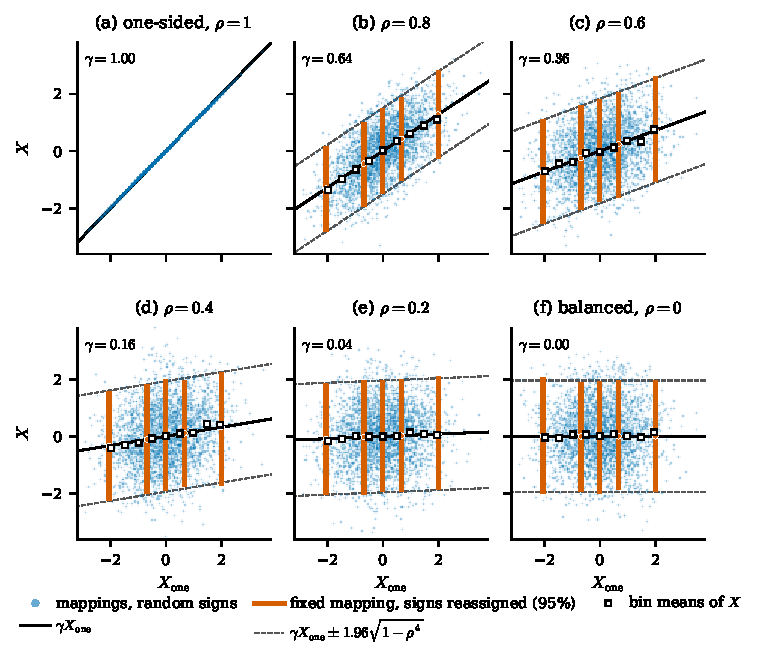
\includegraphics[width=\linewidth]{figures/fig-sign-decomp-all.pdf}
\caption{Decomposition of the graph-conditional sign CLT ($k=3$, $M=16384$, 3000 Plain hypergraphs). Blue points: one random sign assignment per graph; squares: binned means;
orange vertical bars: the 95\% intervals of 5 fixed graphs with signs reassigned on each; dashed lines: $\gamma X_{\rm one}\pm1.96\sqrt{1-\rho^4}$.}
\label{fig:decomp}
\end{figure}

The technical difficulty of the theorem is that fixing the sign composition makes the signs exchangeable but not independent, while the overlap graph
is random, sparse, and irregular, so the existing quadratic form CLTs do not apply directly (Section~\ref{sec:related}).
The proof is in Appendix~\ref{sec:signproof}.

\begin{corollary}[Invariance under balanced selection]\label{cor:balanced}
Under the conditions of Theorem~\ref{thm:sign} let $\rho\to0$. Let the event $\mathcal S$ depend only on the unsigned mapping
and be invariant under element-label permutation. If $\liminf_M\Pr(\mathcal S)>0$, then
\begin{equation*}
\sup_x\left|\Pr(X\le x\mid \mathcal S)-\Phi(x)\right|\longrightarrow0.
\end{equation*}
\end{corollary}
Here $\Phi$ and $\phi$ are the standard normal distribution function and density. Under balanced signs $\gamma\to0$,
the mapping-dependent component $\gamma X_{\rm one}$ of the measurement vanishes, and the remaining $V$ is asymptotically independent of the graph,
so any selection that looks only at the unsigned graph cannot affect it; Figure~\ref{fig:decomp}(f) shows exactly this case. The requirement of a positive lower bound on the probability comes from the precision of asymptotic independence: the dependence of $V$ on $\mathcal G$ vanishes at rate $o(1)$,
and conditioning on an event of vanishing probability can amplify this residual. The sparse-end counterexample of Proposition~\ref{prop:axis} is exactly this situation.
The corollary holds for any positive load limit; it needs no critical-peeling analysis and imposes no rate on $\rho\to0$.
The proof is in Appendix~\ref{sec:signproof}.

Theorem~\ref{thm:sign} hands the role of the sign composition entirely to the factor $\gamma$. The next section then only needs to study the relation between the all-same-sign
$X_{\rm one}$ and the success or failure of peeling, from which the conclusion for general signs follows.
